\documentclass[UTF8,fontset=none,12pt]{ctexart}

\setCJKmainfont{Songti SC}
\setCJKsansfont{PingFang SC}
\setCJKmonofont{Songti SC}

\usepackage[a4paper,margin=2.35cm]{geometry}
\usepackage{amsmath,amssymb,amsthm,mathtools,bm}
\usepackage{graphicx}
\usepackage{float}
\usepackage{booktabs}
\usepackage{array}
\usepackage{enumitem}
\usepackage[hidelinks]{hyperref}

\newcommand{\C}{\mathbb{C}}
\newcommand{\epsmach}{\varepsilon_{\mathrm{machine}}}
\theoremstyle{definition}
\newtheorem{theorem}{定理}
\renewcommand{\thetheorem}{18.\arabic{theorem}}
\renewcommand{\thefigure}{18.\arabic{figure}}

\title{数值线性代数\quad 第 18 讲：最小二乘问题的良态性}
\author{Lloyd N. Trefethen、David Bau III\quad 中文阅读版}
\date{}

\begin{document}
\maketitle
\pagestyle{plain}

最小二乘问题的良态性是一个微妙的主题，它把方程组的良态性与正交投影的几何联系在一起.这一主题之所以重要，是因为它对最小二乘算法的稳定性有并不显然的影响.

\section*{四个良态性问题}

本讲回到线性最小二乘问题 (11.2)，并再次用图 18.1 说明.假设定义问题的矩阵满秩，并且本讲始终使用 2-范数：
\begin{equation}
\begin{gathered}
\text{给定满秩矩阵 }A\in\C^{m\times n},\ m\ge n,\ b\in\C^m,\\
\text{求 }x\in\C^n\text{，使 }\|b-Ax\|\text{ 最小}.
\end{gathered}
\tag{18.1}
\end{equation}

解 $x$ 以及 range$(A)$ 中距离 $b$ 最近的对应点 $y=Ax$ 为
\begin{equation}
    x=A^+b,\qquad y=Pb,
    \tag{18.2}
\end{equation}
其中 $A^+\in\C^{n\times m}$ 是 $A$ 的伪逆 (11.11)，$P=AA^+\in\C^{m\times m}$ 是到 range$(A)$ 上的正交投影.我们将研究问题 (18.1) 对扰动的敏感性.正如上一讲给出了本书最详细的稳定性分析，本讲给出了本书最详细的良态性分析.之所以选择最小二乘问题，是因为其中的细节有趣，而且它有一个重要的实际后果：下一讲将讨论，把正规方程作为通用最小二乘算法会导致不稳定.

\begin{figure}[H]
    \centering
    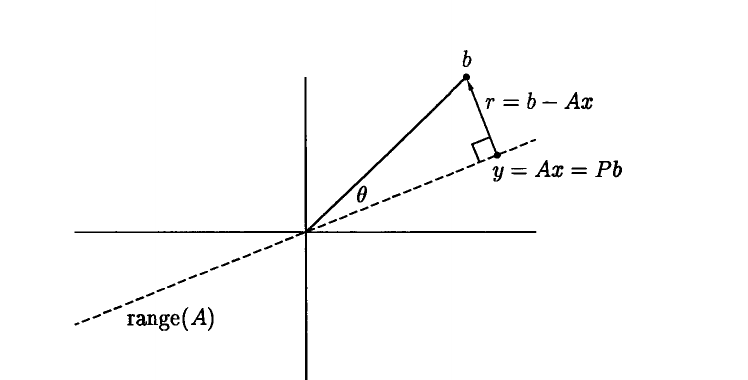
\includegraphics[width=0.78\linewidth]{../assets/figure-18-1.png}
    \caption{最小二乘问题的几何图示（原书图 18.1，重复第 11 讲图 11.3）.}
\end{figure}

良态性描述解对数据扰动的敏感程度.对问题 (18.1)，数据是 $m\times n$ 矩阵 $A$ 和 $m$-向量 $b$；解或者是系数向量 $x$，或者是对应的点 $y=Ax$.因此有两组选择：
\[
\text{数据： }A,b,\qquad \text{解： }x,y.
\]
这两组选择组合起来，就给出了下面将要考虑的四个良态性问题；它们在不同场景中都有应用.

\section*{定理}

本讲的核心是定理 18.1，它回答了上述问题.结论用三个在最小二乘分析中反复出现的无量纲参数表示.

第一个参数是 $A$ 的条件数.对方阵，它是 $\kappa(A)=\|A\|\|A^{-1}\|$；对矩形矩阵，定义推广为 (12.17)：
\begin{equation}
    \kappa(A)=\|A\|\|A^+\|=\frac{\sigma_1}{\sigma_n}.
    \tag{18.3}
\end{equation}

第二个参数是图 18.1 中标出的角 $\theta$，它衡量拟合的接近程度：
\begin{equation}
    \theta=\cos^{-1}\frac{\|y\|}{\|b\|}.
    \tag{18.4}
\end{equation}

第三个参数衡量在给定 $\|A\|$ 和 $\|x\|$ 时，$\|y\|$ 距离最大可能值有多远：
\begin{equation}
    \eta=\frac{\|A\|\|x\|}{\|y\|}=\frac{\|A\|\|x\|}{\|Ax\|}.
    \tag{18.5}
\end{equation}

这些参数满足
\begin{equation}
    1\le\kappa(A)<\infty,\qquad 0\le\theta\le\frac{\pi}{2},\qquad 1\le\eta\le\kappa(A).
    \tag{18.6}
\end{equation}

\begin{theorem}
固定满秩的 $b\in\C^m$ 和 $A\in\C^{m\times n}$.最小二乘问题 (18.1) 中，描述 $b$ 和 $A$ 的扰动对 $y$ 和 $x$ 敏感性的 2-范数相对条件数 (12.5) 如下：
\[
\begin{array}{c|cc}
 & y & x\\
\hline
b & \displaystyle\frac{1}{\cos\theta}
  & \displaystyle\frac{\kappa(A)}{\eta\cos\theta}\\[10pt]
A & \displaystyle\frac{\kappa(A)}{\cos\theta}
  & \displaystyle\kappa(A)+\frac{\kappa(A)^2\tan\theta}{\eta}
\end{array}
\]
第一行的结果是精确的：对某些扰动 $\delta b$ 可以达到；第二行的结果是上界.
\end{theorem}

在特殊情形 $m=n$ 时，问题 (18.1) 退化为方阵非奇异线性系统，此时 $\theta=0$.定理第二列中的数分别化为 $\kappa(A)/\eta$ 和 $\kappa(A)$，正是此前推导的结果 (12.14) 和 (12.18)；左下角的数还可以替换为 0（习题 18.4）.

\section*{化为对角矩阵}

证明定理 18.1 的第一步，是换到一组方便的基，使最小二乘问题更容易分析.设 $A$ 的 SVD 为
\[
A=U\Sigma V^*,
\]
其中 $\Sigma$ 是对角线元素为正的 $m\times n$ 矩阵.由于扰动用 2-范数度量，酉基变换不会改变扰动大小，因此 $A$ 的扰动性质与 $\Sigma$ 相同.所以不妨直接处理 $\Sigma$.以下均假设 $A=\Sigma$，并写成
\begin{equation}
    A=\begin{bmatrix}
    \sigma_1&&\\
    &\ddots&\\
    &&\sigma_n\\
    &&&\\[-6pt]
    &&&
    \end{bmatrix}
    =\begin{bmatrix}A_1\\0\end{bmatrix},
    \tag{18.7}
\end{equation}
其中 $A_1$ 是 $n\times n$ 对角矩阵，$A$ 的其余部分为零.

现在，把 $b$ 写成
\[
b=\begin{bmatrix}b_1\\b_2\end{bmatrix},
\]
其中 $b_1$ 包含 $b$ 的前 $n$ 个分量.此时，将 $b$ 投影到 range$(A)$ 上非常简单：
\[
y=Pb=\begin{bmatrix}b_1\\0\end{bmatrix}.
\]
要找对应的 $x$，将 $Ax=y$ 写为
\[
\begin{bmatrix}A_1\\0\end{bmatrix}x
=\begin{bmatrix}b_1\\0\end{bmatrix},
\]
于是
\begin{equation}
    x=A_1^{-1}b_1.
    \tag{18.8}
\end{equation}
由此可见，正交投影和伪逆分别是如下 $2\times2$ 块矩阵和 $1\times2$ 块矩阵（见习题 11.1）：
\begin{equation}
    P=\begin{bmatrix}I&0\\0&0\end{bmatrix},
    \qquad
    A^+=\begin{bmatrix}A_1^{-1}&0\end{bmatrix}.
    \tag{18.9}
\end{equation}

\section*{$b$ 的扰动对 $y$ 的敏感性}

先看四个良态性结果中最简单的一个.由式 (18.2)，$b$ 与 $y$ 的关系就是线性方程 $y=Pb$.这个映射的 Jacobian 就是 $P$ 本身，由式 (18.9) 有 $\|P\|=1$.因此由式 (12.6) 和 (18.4)，$b$ 的扰动对 $y$ 的条件数为
\[
\kappa_{b\to y}
=\frac{\|P\|}{\|y\|/\|b\|}
=\frac{1}{\cos\theta}.
\]
这就得到定理 18.1 左上角的结果.当 $\delta b$ 除前 $n$ 个分量外均为零时，$\|P(\delta b)\|=\|\delta b\|$，因而这个条件数可以由相应扰动达到.

\section*{$b$ 的扰动对 $x$ 的敏感性}

$b$ 与 $x$ 的关系同样是线性的，即 $x=A^+b$，其 Jacobian 为 $A^+$.由式 (12.6)、(18.4) 和 (18.5)，$b$ 的扰动对 $x$ 的条件数为
\[
\begin{aligned}
\kappa_{b\to x}
&=\frac{\|A^+\|}{\|x\|/\|b\|}
=\|A^+\|\frac{\|b\|}{\|y\|}\frac{\|y\|}{\|x\|}\\
&=\|A^+\|\frac{1}{\cos\theta}\frac{\|A\|}{\eta}
=\frac{\kappa(A)}{\eta\cos\theta}.
\end{aligned}
\]
这就得到定理 18.1 右上角的结果.当 $\delta b$ 满足 $\|A^+(\delta b)\|=\|A^+\|\|\delta b\|=\|\delta b\|/\sigma_n$ 时可以达到这个条件数；这在 $\delta b$ 除第 $n$ 个分量外均为零时发生（如果 $A$ 有多个等于 $\sigma_n$ 的奇异值，也可能有其他分量）.

\section*{倾斜 $A$ 的值域}

对 $A$ 的扰动是非线性的，也更微妙.我们可以用代数方式计算 Jacobian，但这里采用几何观点.注意，$A$ 的扰动会以两种方式影响最小二乘问题：它会扭曲从 $\C^n$ 到 range$(A)$ 的映射，也会改变 range$(A)$ 本身.先考察后一种影响.

我们可以把 range$(A)$ 的微小变化想象成这个空间的轻微“倾斜”.问题是：一个小扰动 $\delta A$ 最多能让这个空间倾斜多大的角度 $\delta\alpha$？答案如下.单位 $n$-球面在 $A$ 下的像是一个平放在 range$(A)$ 中的超椭圆.为了尽可能有效地改变 range$(A)$，我们在超椭圆上取一点 $p=Av$（所以 $\|v\|=1$），并把它沿着正交于 range$(A)$ 的方向推移 $\delta p$.最有效的矩阵扰动是
\[
\delta A=(\delta p)v^*,
\]
因为 $(\delta A)v=\delta p$ 且 $\|\delta A\|=\|\delta p\|$（例 3.6）.

显然，在给定 $\|\delta p\|$ 时，要获得最大倾斜，应使 $p$ 尽可能靠近原点.也就是说，取
\[
p=\sigma_nu_n,
\]
其中 $\sigma_n$ 是 $A$ 的最小奇异值，$u_n$ 是对应的左奇异向量.在对角形式 (18.7) 下，$p$ 就是 $A$ 的最后一列，$v^*$ 是 $n$-向量 $(0,0,\ldots,0,1)$，而 $\delta A$ 是这一列对角线下方条目的扰动.这种扰动使 range$(A)$ 倾斜一个角度 $\delta\alpha$，满足
\[
\tan(\delta\alpha)=\frac{\|\delta p\|}{\sigma_n}.
\]
由于 $\|\delta p\|=\|\delta A\|$ 且 $\delta\alpha\le\tan(\delta\alpha)$，有
\begin{equation}
    \delta\alpha\le\frac{\|\delta A\|}{\sigma_n}
    =\frac{\|\delta A\|}{\|A\|}\kappa(A).
    \tag{18.10}
\end{equation}
对于上述形式的 $\delta A$，只要扰动是无穷小的（从而 $\delta\alpha=\tan(\delta\alpha)$），就能达到等号.

\section*{$A$ 的扰动对 $y$ 的敏感性}

现在可以推导定理 18.1 表格的第二行.先看左侧.由于 $y$ 是 $b$ 到 range$(A)$ 的正交投影，它只由 $b$ 和 range$(A)$ 决定.因此，要研究 $A$ 的扰动对 $y$ 的敏感性，只需研究 range$(A)$ 倾斜某个角度 $\delta\alpha$ 时 $y$ 的变化.

固定 $b$，观察 range$(A)$ 倾斜时 $y$ 的变化，可以看到一个漂亮的几何性质（图 18.2）.无论 range$(A)$ 怎样倾斜，处于其中的向量 $y$ 都必须始终正交于 $y-b$.也就是说，直线 $b-y$ 必须与直线 $0-y$ 垂直.换句话说，调整 range$(A)$ 时，$y$ 会沿着一个球面移动；这个球面的半径是 $\|b\|/2$，球心为 $b/2$.

\begin{figure}[H]
    \centering
    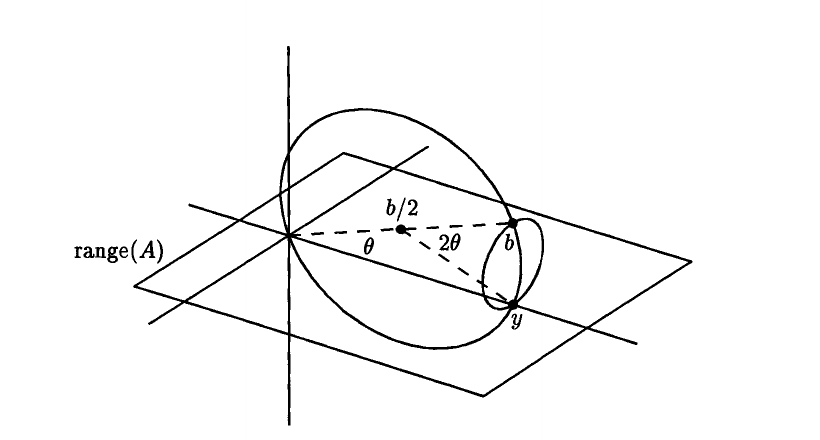
\includegraphics[width=0.88\linewidth]{../assets/figure-18-2.png}
    \caption{当 range$(A)$ 变化时，$y$ 在球面上移动的两个圆.大圆半径为 $\|b\|/2$，对应于在平面 $0$--$b$--$y$ 中倾斜 range$(A)$；小圆半径为 $(\|b\|/2)\sin\theta$，对应于沿正交方向倾斜.无论 range$(A)$ 如何倾斜，$y$ 都留在以 $b/2$ 为球心、半径 $\|b\|/2$ 的球面上.}
\end{figure}

如果在平面 $0$--$b$--$y$ 中将 range$(A)$ 倾斜 $\delta\alpha$，球心 $b/2$ 处的中心角 $2\theta$ 就改变 $2\delta\alpha$.因此，相应的 $\delta y$ 是一个等腰三角形的底边，中心角为 $2\delta\alpha$，两腰长度为 $\|b\|/2$.这说明
\[
\|\delta y\|=\|b\|\sin(\delta\alpha).
\]
沿其他方向倾斜时，几何关系类似，但扰动至少会小一个 $\sin\theta$ 因子.所以对角度为 $\delta\alpha$ 的任意扰动都有
\begin{equation}
    \|\delta y\|\le\|b\|\sin(\delta\alpha)\le\|b\|\delta\alpha.
    \tag{18.11}
\end{equation}
由式 (18.4) 和 (18.10)，得到 $\|\delta y\|\le\|\delta A\|\kappa(A)\|y\|/(\|A\|\cos\theta)$，即
\begin{equation}
    \frac{\|\delta y\|/\|y\|}{\|\delta A\|/\|A\|}
    \le\frac{\kappa(A)}{\cos\theta}.
    \tag{18.12}
\end{equation}
这就得到了定理 18.1 左下角的结果.

\section*{$A$ 的扰动对 $x$ 的敏感性}

现在分析定理 18.1 中最有趣的关系：$A$ 的扰动对 $x$ 的敏感性.

将扰动 $\delta A$ 自然地分成两部分：$A$ 的前 $n$ 行中的 $\delta A_1$，以及剩余 $m-n$ 行中的 $\delta A_2$：
\[
\delta A=\begin{bmatrix}\delta A_1\\\delta A_2\end{bmatrix}
=\begin{bmatrix}\delta A_1\\0\end{bmatrix}
+\begin{bmatrix}0\\\delta A_2\end{bmatrix}.
\]

先考虑扰动 $\delta A_1$.它改变 $A$ 在其值域中的映射，但不改变 range$(A)$ 本身，也不改变 $y$.它在方阵系统 (18.8) 中通过 $\delta A_1$ 扰动 $A_1$，而 $b_1$ 不变.由式 (12.18)，这类扰动的条件数为
\begin{equation}
    \frac{\|\delta x\|/\|x\|}{\|\delta A_1\|/\|A_1\|}
    \le\kappa(A_1)=\kappa(A).
    \tag{18.13}
\end{equation}

接着考虑（无穷小）扰动 $\delta A_2$.它使 range$(A)$ 倾斜，却不改变该空间内 $A$ 的映射.点 $y$ 以及相应的向量 $b_1$ 会发生扰动，但 $A_1$ 不变.这对应于在 (18.8) 中扰动 $b_1$ 而不改变 $A_1$.由式 (12.14)，这类扰动的条件数为
\begin{equation}
    \frac{\|\delta x\|/\|x\|}{\|\delta b_1\|/\|b_1\|}
    \le\frac{\kappa(A_1)}{\eta(A_1;x)}
    =\frac{\kappa(A)}{\eta}.
    \tag{18.14}
\end{equation}

还需要把 $\delta b_1$ 与 $\delta A_2$ 联系起来.向量 $b_1$ 是用 range$(A)$ 的坐标表示的 $y$.因此，只有平行于 range$(A)$ 的 $y$ 的变化，才会表现为 $b_1$ 的变化；正交变化不起作用.特别地，如果在平面 $0$--$b$--$y$ 中把 range$(A)$ 倾斜角度 $\delta\alpha$，那么产生的 $\delta y$ 不平行于 range$(A)$，而是与之成 $\pi/2-\theta$ 角.所以
\[
\|\delta b_1\|=\sin\theta\,\|\delta y\|.
\]
由式 (18.11)，有
\begin{equation}
    \|\delta b_1\|\le(\|b\|\delta\alpha)\sin\theta.
    \tag{18.15}
\end{equation}

有趣的是，如果沿着正交于平面 $0$--$b$--$y$ 的方向倾斜 range$(A)$，仍可得到相同的界，只是原因不同.此时 $\delta y$ 平行于 range$(A)$，但如图 18.2 附近所述，它会小一个 $\sin\theta$ 因子.于是仍有 $\|\delta y\|\le(\|b\|\delta\alpha)\sin\theta$；又因为 $\|\delta b_1\|\le\|\delta y\|$，仍得到式 (18.15).

现在所有部分都已就绪.由于 $\|b_1\|=\|b\|\cos\theta$，式 (18.15) 可以写成
\begin{equation}
    \frac{\|\delta b_1\|}{\|b_1\|}\le(\delta\alpha)\tan\theta.
    \tag{18.16}
\end{equation}
由式 (18.10) 联系 $\delta\alpha$ 与 $\|\delta A_2\|$，再把式 (18.14) 与 (18.16) 合并，得到
\[
\frac{\|\delta x\|/\|x\|}{\|\delta A_2\|/\|A\|}
\le\frac{\kappa(A)^2\tan\theta}{\eta}.
\]
将这个界与式 (18.13) 相加，就得到定理 18.1 右下角的结果.

\section*{习题}

\begin{enumerate}[label=\textbf{18.\arabic*}]
    \item 考虑例子
    \[
    A=\begin{bmatrix}1&1\\1&1.0001\\1&1.0001\end{bmatrix},
    \qquad
    b=\begin{bmatrix}2\\0.0001\\4.0001\end{bmatrix}.
    \]
    \begin{enumerate}[label=(\alph*)]
        \item 求这个例子的矩阵 $A^+$ 和 $P$.给出精确答案.
        \item 求最小二乘问题 $Ax\approx b$ 的精确解 $x$ 和 $y=Ax$.
        \item 求 $\kappa(A)$、$\theta$ 和 $\eta$.从这里开始，数值答案即可.
        \item 求定理 18.1 中的四个条件数.
        \item 给出扰动 $\delta b$ 和 $\delta A$ 的例子，使它们近似达到这四个条件数.
    \end{enumerate}

    \item 社会科学家依赖回归技术：用其他向量的线性组合，以最小二乘意义近似某个量的观测向量.拟合系数随后被解释为 IQ、受教育年限、父母受教育年限和父母收入等因素对年收入的影响.人们可能以为，在模型中加入越多变量，就能获得越多信息，但事实并不总是如此.请从良态性的角度解释这一现象，并明确联系定理 18.1 的结果.

    \item 假设你隔着 Cayuga 湖看向对岸房屋发出的灯光.如果湖面有波纹，反射光会呈现一条很长的竖直光带.雨天道路上前车的尾灯，或者打蜡地板上走廊灯的反射，也会出现同样的现象.这是真实的几何效应，而不是视觉错觉.
    \begin{enumerate}[label=(\alph*)]
        \item 建立一个解释这一现象的定量理论.具体地，假设你和湖对岸的房屋都在水面上方 50 米处，湖宽为 1 千米.在你的视野中，光带的长宽比是多少？
        \item 描述这个问题与本讲某个几何论证之间的联系.
    \end{enumerate}

    \item 解释为什么正如定理 18.1 后所述，当 $m=n$ 时，$y$ 对 $A$ 扰动的条件数变为 0.
\end{enumerate}

\end{document}
